\section{Tilpasning af træningsniveau}
I tilpasningscontrolleren beregnes den anbefalede træningstid. Dette gøre ud fra kategorisering, den daglige helbredstilstand og en tidligere evaluering, foretaget efter samme træningsform, -type og helbredstilstand.
Beregningen for den anbefalede træning er implementeret ved brug af if/else-statement. Et udpluk af denne beregning fremgår af \autoref{fig:anbekode}.  
   
\begin{figure} [H]
\centering
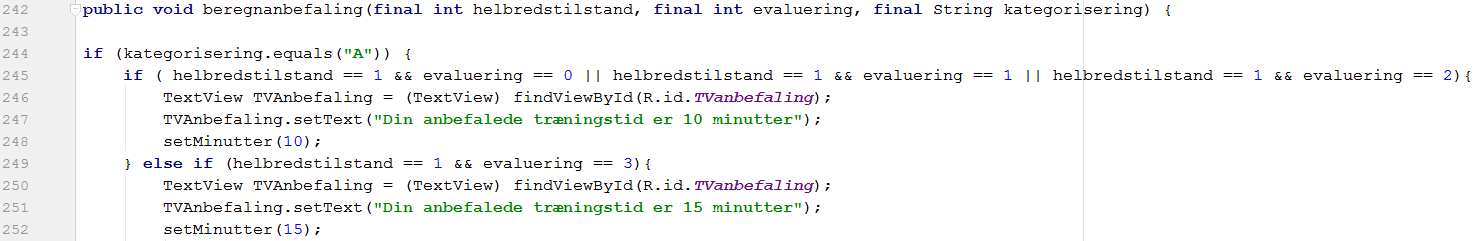
\includegraphics[width=1\textwidth]{figures/imple/anbekode}
\caption{Udpluk af koden for anbefalet træning. If/else-loops afgør, hvilket træningsniveau brugeren får anbefalet.}
\label{fig:anbekode}
\end{figure} 

\noindent
Af figuren ses beregningen af den anbefalede træningstid for brugeren med kategorisering \textit{A} og heldbredstilstanden på \textit{2}. Variationen for anbefalingen afhænger af evalueringen og kan i dette eksempel variere mellem \textit{15}, \textit{20} og \textit{25}  minutter. Metodekaldet, \textit{setMinutter}, refererer til, at der sættes en bemærkning, idet den anbefaldede træningstid er opnået.

\section{Træning}
Træningscontrolleren har til formål at håndtere GPS-lokalisation for at beregne tilbagelagt afstand under træning. Ligeledes håndterer controlleren en timer, der viser tiden brugt til den givne træning. Efter træningen er udført, vil træningscontrolleren opsætte en notifikation som efterfølgende vises dagligt. 


\subsection*{Afstandsberegning}
For at implementere GPS skal app'en have tilladelse til at anvende den mobile enheds lokalisation. Dette er en engangstilladelse, der skal gives første gang brugeren vil foretage en træning. 

Der instansieres en LocationManager og LocationListener. LocationManager tillader app'en at opnå enhedens lokalisation, hvor LocationListener modtager lokalisationsopdateringer. Disse opdateringer forekommer, idet enheden ændrer lokalisation.\cite{LocationManager, LocationListener} Af koden i \autoref{fig:gpsKode} fremgår det, at systemet indeholder en metode, \textit{onLocationChanged}, der kaldes, når lokalisationen ændres. 

\begin{figure} [H]
\centering
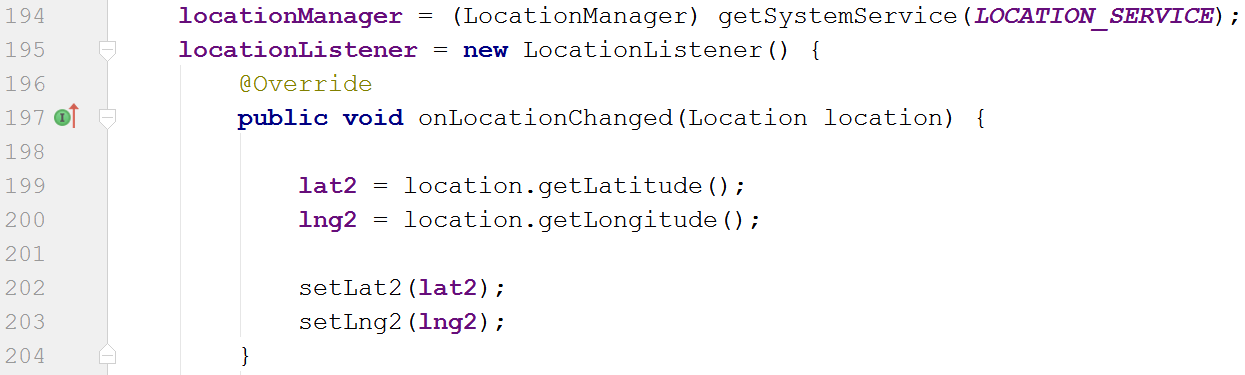
\includegraphics[width=1\textwidth]{figures/imple/gpsKode}
\caption{Metoden, onLocationChanged, der kaldes, når lokalisation ændres.}
\label{fig:gpsKode}
\end{figure} 

\noindent
Når lokalisationen ændres, hentes enhedens longitude og latitude, hvortil disse værdier benyttes i set-metoder. Afstanden beregnes ud fra følgende formel:
\begin{equation} \label{equ:GPS}
d = \arccos(\sin(lat_1)*\sin(lat_2)+\cos(lat_1)*\cos(lat_2)*\cos(lon_2-lon_1))*R
\end{equation}

\noindent
Formlen, der ses af \autoref{equ:GPS}, benyttes til at udregne afstand ud fra to longitude- og latitudepunkter. Af formlen betegner \textit{d} den udregnede afstand, \textit{$lat_1$}, \textit{$lon_1$} samt \textit{$lat_2$}, \textit{$lat_2$} er latitude- og longitudekoordinaterne for henholdsvis den første og anden lokalisation. \textit{R} betegner jordens radius.\cite{Deza2009}    

Ligning \ref{equ:GPS} implementeres i javakode, hvortil denne benytter longitude- og latitudekoordinaterne, der hentes fra koden, som ses af \autoref{fig:gpsKode}. Implementeringen af formlen ses af \autoref{fig:distanceKode}.

\begin{figure} [H]
\centering
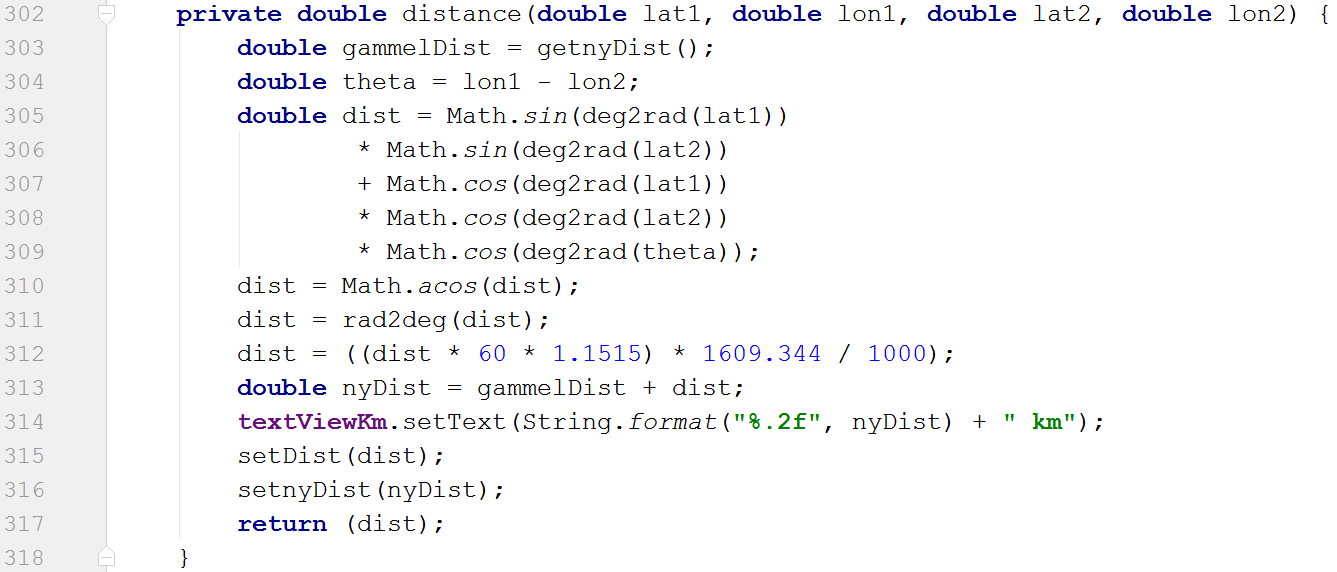
\includegraphics[width=1\textwidth]{figures/imple/distanceKode}
\caption{Metode i træningscontrolleren, der beregner afstanden i kilometer ud fra lokalisationer.}
\label{fig:distanceKode}
\end{figure}
 
\noindent
Metoden, \textit{distance}, kaldes hver gang, der sker en lokalisationsændring og beregner afstanden mellem enhedens pågældende lokalisation samt forrige lokalisationsopdatering. Af koden fremgår det, at latitude- og longitudeværdierne konverteres fra grader til radianer for at kunne anvende cosinus- og sinusfunktionerne. 
Afstanden ønskes udregnet i kilometer, hvortil \textit{dist} ganges med jordens radius i kilometer. 
Efterfølgende sættes den udregnede totale afstand \textit{nyDist}, hvortil denne værdi hentes og gemmes i variablen \textit{gammelDist}.   


\subsection*{Timer}
I træningscontrolleren startes en timer for at kunne monitorere træning. Denne er implementeret ved at instansiere klassen \textit{Runnable}, hvori en metode, \textit{run}, defineres. Koden for dette kan ses i \autoref{fig:timerKode}.

\begin{figure} [H]
\centering
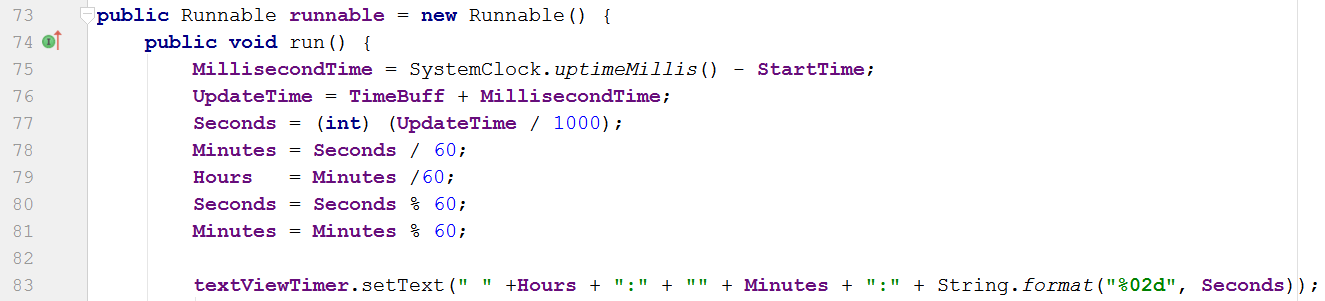
\includegraphics[width=1\textwidth]{figures/imple/timerKode}
\caption{Udklip af kode fra træningscontrolleren. Udklippet viser metoden for timeren.}
\label{fig:timerKode}
\end{figure} 

\noindent
Metoden, \textit{run}, indeholder variablen \textit{MillisecondTime}, der tæller tiden, som er gået siden brugeren har trykket start træning. Vælger brugeren at trykke stop træning, stopper \textit{MillisecondTime} med at tælle op, hvortil denne værdi gemmes i variablen \textit{TimeBuff}.  Værdien gemmes for, at timeren vil kunne fortsætte, hvis brugeren ønsker at fortsætte træningen. \textit{Seconds} defineres ud fra \textit{UpdateTime}, der måles i millisekunder. Det defineres yderligere, at \textit{Seconds} kun kan tælle op til 60.

Under tilpasning af træningsniveau er der blevet anbefalet en træningstid. Opnår træningstiden denne værdi under træning, vil app'en gøre brugeren opmærksom på dette ved angivelse af en lyd. Dette er implementeret ved en if-loop, hvori klassen MediaPlayer instansieres, hvis den anbefalede tid opnås. Hertil kaldes en metode, der afspiller en lydfil. 


\subsection*{Notifikation}
Ifølge de opstillede kravspecifikationer skal app'en sende en daglig notifikation. Denne er implementeret i træningscontrolleren, hvor notifikationen aktiveres første gang brugeren har evalueret en træning. Hertil er det implementeret, ved brug af klassen \textit{Calendar} og metoden \textit{getInstance}, at den daglige notifikation sendes klokken 15. Af \autoref{fig:notifikationKode} fremgår et udklip af koden, som definerer tidspunktet for notifikationen. 

\begin{figure} [H]
\centering
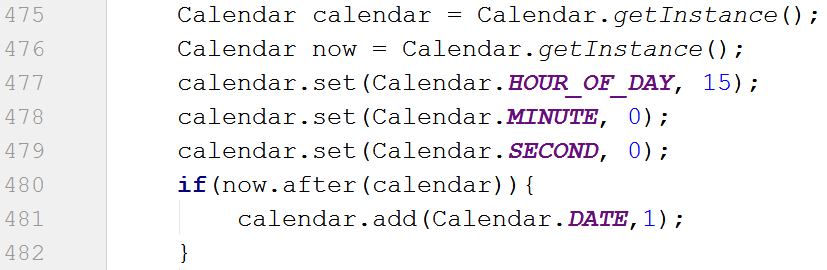
\includegraphics[width=0.7\textwidth]{figures/imple/notifikationKode}
\caption{Udklip af kode fra træningscontrolleren, som viser notifikationens starttidspunkt.}
\label{fig:notifikationKode}
\end{figure} 
